\documentclass[tikz]{standalone}
%\'{a}\^{g} ki di-ta nu-\^{g}en-\'{a}\^{g} ki --eme-gir$_\text{7}$ qa-b\^{u}m
%You are not one who stays in one place, you are one who is everywhere. --Sumerian Saying

\tikzset{
    wedge/.pic={
        \filldraw (0,2) -- (1.5,3.5) .. controls (0.8,2.2) and (1.4, 1) .. (2.25,0) -- cycle;
    },
    stick/.pic={
        \filldraw (0,5) .. controls (0.9,4) .. (1,0) .. controls (1.1,4.2) .. (2,5) .. controls (0.9,4.7) .. (0,5);
    }
}

\begin{document}
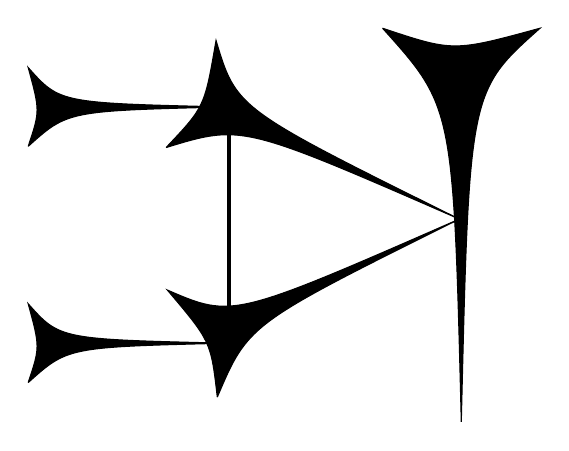
\begin{tikzpicture}
    %ki
%    \begin{scope}
%    \pic at (2.5,0) [rotate=40] {stick};
%    \pic at (-4.5,1.5) [rotate=-40] {stick};
%    \pic at (-1,-3) [rotate=50] {stick};
%    \pic at (-1,-1.5) [rotate=-50] {stick};
%    \pic at (1.7,1.8) [yscale=0.6,xscale=0.65,rotate=90] {stick};
%    \pic at (2.6,0.8) [yscale=0.6,xscale=0.82,rotate=90] {stick};
%    \pic at (2.5,-0.2) [yscale=0.6,xscale=0.8,rotate=90] {stick};
%    \pic at (1.75,-1.2) [yscale=0.6,xscale=0.65,rotate=90] {stick};
%    \end{scope}
    %di
    %\begin{scope}
%    \pic at (2.5,0) [rotate=40] {stick};
%    \pic at (-4.5,1.5) [rotate=-40] {stick};
%    \pic at (-1,-3) [rotate=50] {stick};
%    \pic at (-1,-1.5) [rotate=-50] {stick};
%    \pic at (2.6,0.65) [yscale=0.8,xscale=0.82,rotate=90] {stick};
%    \pic at (2.5,-0.7) [yscale=0.8,xscale=0.8,rotate=90] {stick};
%    \end{scope}
    %ta
    \begin{scope}
    \pic at (-2.3,3.5) [rotate=90, scale=0.5] {stick};
    \pic at (-2.3,0.5) [rotate=90, scale=0.5] {stick};
    \pic at (1,1.9) [scale=0.75,rotate=115] {stick};
    \pic at (0.35,1.9) [scale=0.75,rotate=65] {stick};
    \pic at (-0.3,0) {stick};
    \draw [very thick] (-2.25,1) -- (-2.25,4);
    \end{scope}
    %nu
%    \begin{scope}
%    \pic at (4.5,2.55) [rotate=90] {stick};
%    \pic at (0,0) {stick};
%    \pic at (5.2,2.8) [rotate=135] {stick};
%    \end{scope}
    %\^{g}en
%    \begin{scope}[xshift=5cm]
%    \pic at (-1,2.55) [rotate=90, scale=0.65] {stick};
%    \pic at (-1.7,2) [scale=0.6] {wedge};
%    \pic at (-2.3,0.5) [rotate=90, scale=0.5] {stick};
%    \pic at (0,0.5) [rotate=90, scale=0.5] {stick};
%    \pic at (-1,0) {stick};
%    \end{scope}
\end{tikzpicture}
\end{document} 